\chapter{Sprint 4 --- Evaluation and Release Readiness}
\chaptermark{Sprint 4 --- Evaluation \& Readiness}
\label{chap:sprint-4}

This chapter presents the realization of Sprint 4, the internship's
final sprint: consolidating Sprints 1--3's pipeline into a coherent,
evaluable, demoable product rather than adding new pipeline stages,
covering the sprint's backlog, design, implementation, testing, and
review.

\section{Sprint Goal}

\begin{quote}
Every earlier page rebuilt on the real design system, the system's
actual quality proven in real, regression-gated evaluation numbers
rather than asserted, and a release-readiness package showing it end to
end.
\end{quote}

Sprint 4 ran July 27--31, 2026, with 35 points committed, the smallest
sprint by design. This was a deliberate wind-down, not a loss of momentum:
Sprint 3 already closed the last core-pipeline story on the product
backlog (Conclusion, Section~\ref{sec:s3-conclusion}), so Sprint 4's entire
capacity could be reallocated toward proving what already existed:
polish, evaluation rigor, observability, a first privacy pass, and a
release-readiness validation package, rather than further system
capability.

\section{Sprint Backlog}

Table~\ref{tab:sprint4-backlog} lists Sprint 4's committed stories, points, and status.

\begin{table}[H]
  \centering
  \caption{Sprint 4 backlog}
  \label{tab:sprint4-backlog}
  \begin{tabular}{@{}p{1.7cm}p{11.2cm}p{1.3cm}p{2.7cm}@{}}
    \toprule
    ID & Story & Points & Status \\
    \midrule
    ADQ-26 & Enterprise-grade UX/UI overhaul of every Sprint 1--3 page & 5 & Done \\
    ADQ-27 & Metrics dashboard presenting real evaluation numbers to both reviewers and maintainers & 5 & Done \\
    ADQ-28 & First-run guided product tour & 3 & Done \\
    ADQ-29 & Automated faithfulness/groundedness scoring, an LLM-judge safeguard confirming every generated rationale is actually backed by evidence & 5 & Done \\
    ADQ-30 & CI regression suite gating extraction and faithfulness quality & 5 & Done \\
    ADQ-31 & End-to-end LangSmith tracing completed across the worker process boundary & 2 & Done \\
    ADQ-32 & Lightweight local PII pre-processing, masking contact details and candidate names before any external LLM call & 5 & Done \\
    ADQ-33 & Final evaluation pass and release-readiness validation package & 5 & Done \\
    \bottomrule
  \end{tabular}
\end{table}

All 35 points shipped within the sprint window.

\section{Analysis}

The eight stories decompose into three concerns, each building on the
system Sprints 1--3 already delivered:

\begin{description}
  \item[Dashboard and onboarding] (ADQ-26, ADQ-28): every earlier page
    (candidate upload, TDR upload/breakdown) was functional but visually
    unfinished, built on bare HTML with no consistent design system; a
    new user also had no guided entry point into the system's actual
    workflow.
  \item[Evaluation and release-readiness rigor] (ADQ-27, ADQ-29, ADQ-30,
    ADQ-33): earlier sprints produced claims (``the anomaly detector
    works,'' ``the rationale is faithful to the source'') without a
    single place presenting them as real, measured, regression-gated
    numbers. This is the sprint's largest single concern by points (20 of
    35): treating measurement as a first-class deliverable, not an
    afterthought, is standing engineering practice on this project, not
    a bar lowered because it happens to be an internship's final sprint.
  \item[Observability and a first privacy pass] (ADQ-31, ADQ-32): two
    real, independent gaps: no way to inspect what happened inside a
    given pipeline run beyond application logs, and no safeguard at all
    against sending a candidate's name, phone number, or email to an
    external LLM provider.
\end{description}

\section{Design}

Three diagrams and one data contract cover Sprint 4's design: the use
case gained this sprint (a second actor, alongside the returning
HR/bid manager), the boundary where PII masking sits in front of every
external LLM call, the sequence that boundary and end-to-end tracing
take together on one call, and the read-only metrics snapshot schema the
dashboard renders. Sprint 4 introduces no new domain models or pipeline
nodes, so this section is proportionally lighter than Sprints 2--3's.

\subsection{Use Case Diagram}
\label{sec:s4-usecase}

Figure~\ref{fig:s4-usecase} introduces a second actor alongside the
returning HR/bid manager: the maintainer, the technically literate
colleague (an IT admin, a developer, ST2i's own team) who keeps the
system healthy rather than uses it to staff a bid. Following the guided
tour, viewing system metrics, and inspecting a pipeline trace are the
genuinely new interactions this sprint adds, the latter two specifically
for the maintainer; every Sprint 1--3 page also received the same UX/UI
overhaul (ADQ-26), noted on the diagram rather than modeled as its own
use case, since a visual refresh is not a new interaction.

\begin{figure}[H]
  \centering
  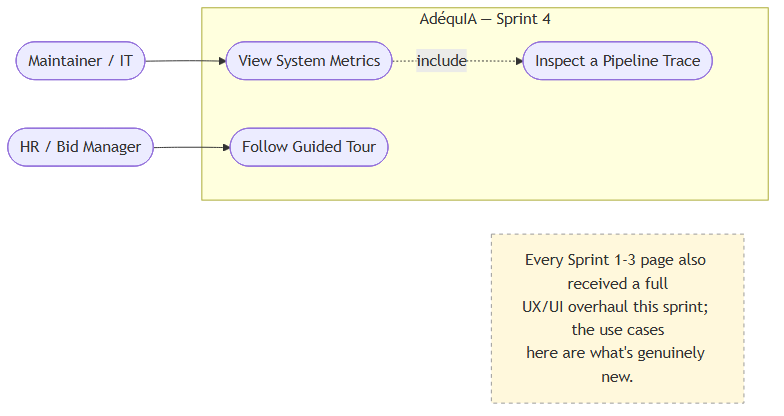
\includegraphics[width=0.85\textwidth]{s4-usecase.png}
  \caption[Sprint 4 use case diagram]{Sprint 4 use case diagram: the HR/bid manager and a new maintainer actor.}
  \label{fig:s4-usecase}
\end{figure}

\subsection{PII Masking Placement}
\label{sec:s4-pii-design}

Figure~\ref{fig:s4-pii} places masking upstream of the routing decision
itself, not conditioned on which provider ends up serving the call. A CV
or TDR's raw extracted text reaches \texttt{app/common/pii.py}'s
\texttt{mask\_pii(text)} \emph{before} the message is even built, which
is in turn before \texttt{ModelRouter} ever decides whether a Groq/Gemini
key is live or every key in both pools is exhausted (Development
Environment, Section~\ref{sec:dev-environment}): \texttt{ModelRouter}
only ever receives the messages it is handed, already masked, so the
same masked text reaches a local Ollama fallback too, not just Groq or
Gemini. Masking runs three passes in order: email and phone detection
(phone patterns only trusted adjacent to an email or an explicit label
such as ``t\'el:'', to avoid false positives like French-formatted
numbers inside ordinary sentences), then name detection (an explicit
label, or a line immediately above an already-masked email/phone,
filtered against a job-title word list so a role like ``Chef de Projet''
is never masked as a person's name). Masked text, not the original, is
what every downstream extraction/scoring/report-generation node actually
sends to \texttt{ModelRouter}; masking happens once, at the boundary,
not repeated per call site.

\begin{figure}[H]
  \centering
  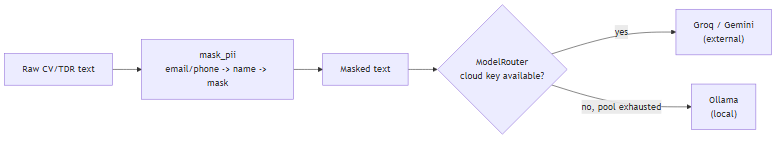
\includegraphics[width=0.9\textwidth]{s4-pii-masking.png}
  \caption[PII masking placement]{PII masking sits before routing is
  decided; both the cloud and local-fallback paths receive the same
  masked text.}
  \label{fig:s4-pii}
\end{figure}

\subsection{Sequence: An External LLM Call, Masked and Traced}
\label{sec:s4-sequence}

Figure~\ref{fig:s4-sequence} follows one call end to end, tying ADQ-31
and ADQ-32 together: the node hands its raw text to \texttt{mask\_pii}
before \texttt{ModelRouter} ever sees it, so by the time
\texttt{ModelRouter} decides between a live Groq/Gemini key and a local
Ollama fallback, both branches are already working with the same masked
text, not a raw one reserved for the local path; either branch's result
is logged to LangSmith with input, output, and latency, closing the one
gap ADQ-31 found (Implementation, Section~\ref{sec:s4-impl}).

\begin{figure}[H]
  \centering
  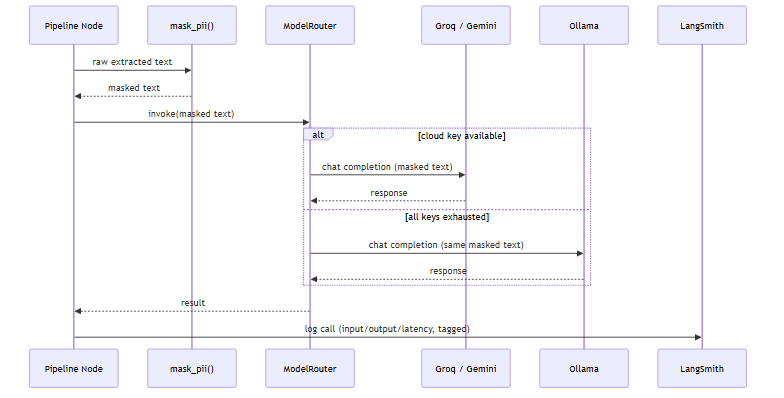
\includegraphics[width=0.85\textwidth]{s4-sequence.png}
  \caption[Sprint 4 masked/traced call sequence]{Sprint 4 sequence: masking happens before routing, so both the cloud and local-fallback branches are traced on the same masked text.}
  \label{fig:s4-sequence}
\end{figure}

\subsection{Metrics Snapshot}

The metrics dashboard (ADQ-27) does not compute anything live. It reads
a single JSON snapshot file
(\texttt{backend/app/features/metrics/current\_snapshot.json}) produced by
the real eval suites (ADQ-29, ADQ-30, ADQ-33), exposed through one
read-only endpoint, \texttt{GET /metrics}. Each of the seven metric
groups (extraction, retrieval, anomaly detection, guardrails, scoring
agreement, report quality, efficiency) carries its own \texttt{status}
(\texttt{available}/\texttt{pending}), \texttt{dataset},
\texttt{sample\_size}, and an optional \texttt{note}, so a metric that
is honestly not yet measurable renders as a stated gap on the dashboard,
not a missing row or a fabricated number.

\section{Implementation}
\label{sec:s4-impl}

Each backlog story is covered in turn, including two data-honesty
defects live use of the new dashboard itself surfaced along the way.

\subsection{ADQ-26 Enterprise-Grade UX/UI Overhaul}

Candidate and TDR pages were rebuilt on shadcn/ui (Radix primitives),
moving the product off bare, unstyled HTML and onto the same
component system enterprise SaaS products are typically built on: real
empty states that explain what to do next rather than showing a blank
list, tooltips on non-obvious concepts (hard-filter vs. scored criteria,
anomaly severity), and consistent table/card layout across every page.
This is a UX decision as much as a visual one, since Radix's primitives
carry keyboard navigation and screen-reader semantics for free rather
than needing them retrofitted later. Live testing during this story
surfaced a real data bug, not a styling one: a pre-migration
content-hash column had never been backfilled for rows that existed
before it was introduced, producing spurious duplicate rows in the
candidate/TDR lists once the new list views made the duplication
visually obvious for the first time. It was root-caused and fixed with a
regression test, not hidden by the new styling.

\subsection{ADQ-27 Metrics Dashboard for Reviewers and Maintainers}

A metrics page is not something every internal tool needs; it earns its
place here because AdéquIA now serves two real audiences (Design,
Section~\ref{sec:s4-usecase}): the HR/bid manager, who wants a plain
read on whether the system's outputs can be trusted, and the maintainer,
who wants the dataset and sample size behind every number.
\texttt{frontend/src/app/metrics/page.tsx} serves both from the same
seven cards: each renders its real values (or, for a \texttt{pending}
group, a stated reason it is not measured yet) behind a plain-language
tooltip explanation, with the eval dataset and sample size the number
came from always visible alongside it, since a number without its
provenance was treated as worse than no number at all. A second defect
was found and fixed the same way as ADQ-26's: the
Education/Experience/Certification/Language sub-score bars were rendering
an intentional \texttt{null} as a fake 0\%, because the frontend was
coalescing \texttt{null} to \texttt{0} on display: these four sub-scores
were never wired to a real computation in this project (a separate
concern from the pass/fail hard filters of the same names), and leaving
them null was always the honest choice over a fabricated number. The fix
was a pure frontend rendering change; nothing in the backend's scoring
logic was wrong, but an honest \texttt{null} was being displayed as a
failing score on every single match report until this was caught by
direct use of the new dashboard.

\subsection{ADQ-28 First-Run Guided Tour}

A skippable walkthrough (\texttt{driver.js}) highlighting
\texttt{data-tour}-tagged elements in sequence: upload a TDR, see its
extracted positions, run matching, read a ranked shortlist, open a full
report, understand a flagged anomaly, and use the approve/reject/override
controls. This is progressive disclosure, a deliberate onboarding
pattern rather than decoration: instead of a static help page a
first-time reviewer has to go find on their own, the tour meets them
inside the same end-to-end path they will actually use, one step at a
time, so the whole system is understood, not just whichever page they
happened to land on first.

\subsection{ADQ-29 \& ADQ-30 Faithfulness Scoring and a CI Regression Gate}

Faithfulness (also called groundedness) is a standard LLM-evaluation
concept: does every claim a model writes actually trace back to a real
source, or did it quietly embellish beyond what the evidence supports?
Report faithfulness here is judged with RAGAS (an open-source
LLM-output evaluation framework), by a second LLM call scoring each
claim in a generated rationale against its own citation-ledger entry,
never the raw CV/TDR text, the same boundary \texttt{generate\_report}
itself is guardrailed to (ADQ-22): an LLM-as-judge pattern, not a
hand-checked spreadsheet. This is a genuine functional safeguard, not a
cosmetic add-on to this sprint's dashboard work: it is what lets the
system's own claim, ``the rationale is faithful to the source,'' be
checked rather than taken on faith. Live testing this story caught and
fixed a real prompt gap: \texttt{generate\_report}'s guardrail had been
allowing embellishing detail beyond what a cited fact actually
supported; faithfulness went from failing to \textbf{0.91} (10 of 11
judged claims fully backed) once the prompt was tightened. A
DeepEval-based CI regression gate (\texttt{eval.yml}, manually triggered
per Development Environment, Section~\ref{sec:dev-environment}) fails
the build if extraction F1 (the precision/recall harmonic mean,
Section~\ref{sec:s3-adq21}) drops more than 3 points, or faithfulness
drops below 0.85, against the gold sets (hand-verified reference
datasets an eval is scored against, distinct from any live production
sample): protecting a number that already exists from silently
regressing, not producing the number itself.

\subsection{ADQ-31 Completing End-to-End Tracing}

LangSmith tracing had been configured in the API process since an
earlier sprint, but every real pipeline call actually executes in the RQ
background worker, a separate process tracing had never reached (Design,
Section~\ref{sec:s4-sequence} shows the same masked call now logged on
both the cloud and local-fallback branch). This story extended tracing
across that process boundary: every node call is now traced with
input/output/latency, tagged by \texttt{tdr\_id}/\texttt{position\_id},
so one full multi-candidate matching run is viewable as a single trace
group.

\subsection{ADQ-32 PII Pre-Processing}

Implementation matches the Design section above (Section~\ref{sec:s4-pii-design}).
Concretely, three regex passes run over the text before it ever reaches
a cloud provider: an email pattern catches any address outright; a
phone pattern only fires on a line that also carries an already-masked
email or an explicit label such as ``t\'el:''/``gsm:'' -- a bare ``16
500 jeunes'' (a population figure from a real TDR fixture) was wrongly
masked as a phone number before this gating was added, since a French
thousands-separated number shares the exact shape of a local phone
number; and a name pattern matches a capitalized 2--4 word line near the
top of the document, filtered against a job-title word list so a
headline like ``Chef De Projet Senior'' is never masked as the
candidate's own name. In practice, a line such as ``Amine Ferjani --
amine.ferjani@example.com -- +216 23 147 963'' becomes ``[NOM] --
[EMAIL] -- [PHONE]'' before it ever leaves the machine. Worth stating
plainly, as the project's own documentation does: this is deliberately
\emph{lightweight, regex-based masking}, not full compliance-grade
redaction: a real, honest first mitigation given the constraint (an
unpaid internship's zero-budget, free-tier-only infrastructure sending
text to providers outside ST2i's control), not a claim of complete PII
protection.

\subsection{ADQ-33 Final Evaluation Pass and Release-Readiness Validation}

Every evaluation metric tracked for this project was computed with real
numbers, each documented next to the dataset and sample size it came
from (Table~\ref{tab:final-metrics}). Cohen's $\kappa$, the statistic
used for scoring agreement, corrects raw percent agreement for the rate
two independent decision-makers would agree on by pure chance, so a high
value reflects genuine alignment rather than coincidence; here it
compares the AI's hard-filter recommendation against the real reviewer's
decision. The two honestly incomplete figures, TDR field-level F1 and
the $n{=}2$ scoring-agreement sample, are called out rather than hidden:
see the Retrospective (Section~\ref{sec:s4-retro}) for the former.

\begin{table}[H]
  \centering
  \caption{Final evaluation results}
  \label{tab:final-metrics}
  \begin{tabular}{@{}p{3.6cm}p{2.4cm}p{11.0cm}@{}}
    \toprule
    Metric & Result & Dataset / notes \\
    \midrule
    CV extraction F1 & 0.978 & 11 real synthetic CVs, hand-checked \\
    TDR extraction (doc.\ pass-rate) & 92.3\% & 12/13 real TDR PDFs; field-level F1 still a placeholder \\
    Retrieval Recall@3 & 1.0 & One true match per position \\
    Retrieval Precision@3 & 0.33 & Expected at $k{=}3$ with one true match \\
    Anomaly detection P/R/F1 & 1.0 & 0\% false positives, 4 rule-based types \\
    Injection resistance & 100\% (5/5) & One real vulnerability found and fixed \\
    Report faithfulness & 0.91 & LLM-as-judge against citation ledger \\
    Citation coverage & 1.00 & Same 11 judged claims as faithfulness above \\
    Scoring agreement (Cohen's $\kappa$) & 1.0 & $n{=}2$ real reviewer decisions, honestly small \\
    Efficiency, median & 3.52s & Per candidate--position match \\
    Efficiency, p95 & 4.65s & Per candidate--position match \\
    Cost & \$0 & Free-tier-only architecture (Groq/Gemini free tier + local Ollama) \\
    Cost, Claude Sonnet 5 equivalent & \$0.08 (est.) & Estimated, not measured: this sprint's own 28-call efficiency benchmark (Testing, Section~\ref{sec:s4-testing}; 2 real TDR PDFs, 2 real synthetic CVs) re-tokenized with \texttt{tiktoken} against the real system prompts and priced at Sonnet 5's published \$2/\$10 per MTok rate; upper bound, assumes every pair clears the hard filter \\
    \bottomrule
  \end{tabular}
\end{table}

Beyond the metrics themselves, this pass assembled the
release-readiness assets the numbers above feed into: a real LangSmith
trace capture (Sprint Review, Section~\ref{sec:live-demo-sprint4}), the
compiled table above, and a scripted walkthrough validating the system
end to end on real anonymized data, each built directly from
ADQ-27/29/30/31's own outputs rather than written independently of
them.

\section{Testing}
\label{sec:s4-testing}

Sprint 4 added no new pipeline nodes, so the backend unit suite's growth
this sprint is smaller than Sprints 2--3's, concentrated on the new PII
masking regex logic (including the false-positive cases found during
manual testing against a real TDR) and the metrics-endpoint/snapshot
schema. The eval-tier suites (\texttt{pytest -m eval}, real LLM calls,
never part of the default run) grew to cover faithfulness scoring
directly and to formalize the CI regression gate thresholds. Every
number reported in ADQ-33 above was produced by one of these real,
LLM-calling eval runs, not estimated or hand-typed.

\section{Sprint Review}

The sprint was demoed against its own goal: a fully styled dashboard
across every page, a metrics page presenting Sprint 1--4's real,
measured numbers rather than a placeholder, a first-run guided tour, and
a live, traced, PII-masked pipeline run shown end to end.

\subsection{Live Demonstration}
\label{sec:live-demo-sprint4}

% TODO: these three are still PLACEHOLDER images (generated by
% notes/generate_placeholders.py), not real screenshots -- replace the
% files in docs/report/assets/screenshots/ with real captures using
% these exact filenames before this report ships. The \includegraphics
% blocks and captions below are already wired up for the real content.

Figure~\ref{fig:metrics-dashboard} is the metrics dashboard: the seven
evaluated metric groups (ADQ-33) as charts, each with its dataset and
sample size stated alongside it, not a bare number.

\begin{figure}[H]
  \centering
  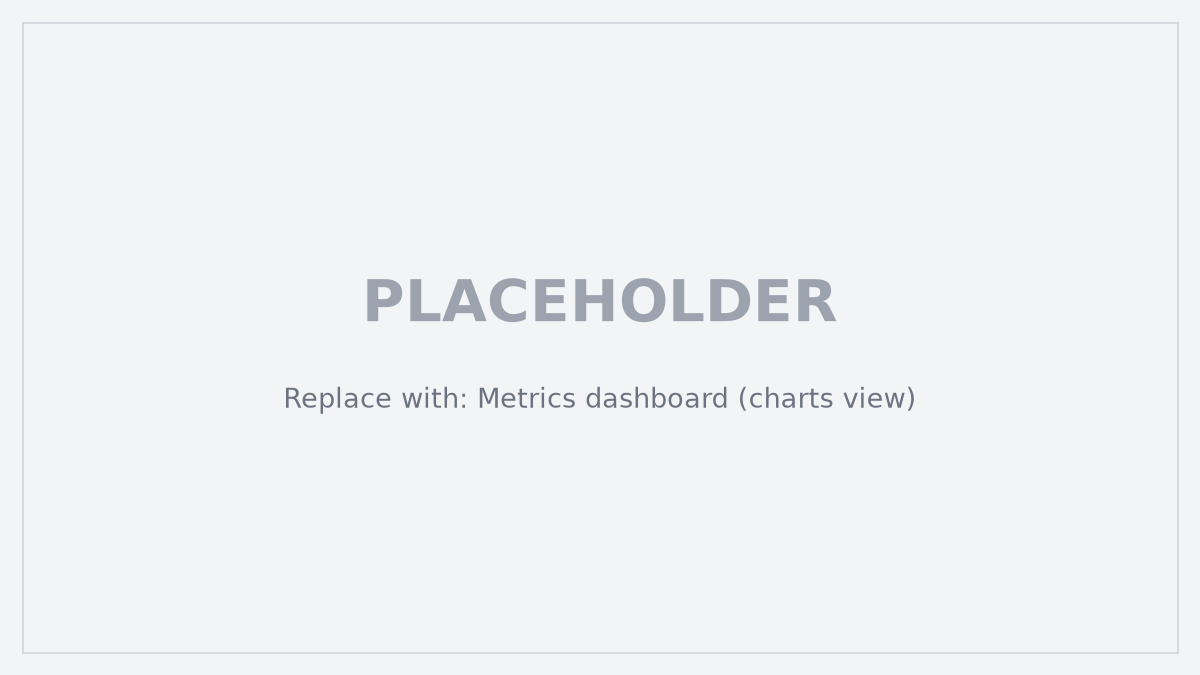
\includegraphics[width=0.75\textwidth]{metrics-dashboard-charts.png}
  \caption[Metrics dashboard]{Metrics dashboard: evaluated metric
  groups as charts.}
  \label{fig:metrics-dashboard}
\end{figure}

Figure~\ref{fig:guided-tour} is the first-run guided tour (ADQ-28)
mid-sequence, highlighting one step of the upload-to-review workflow
with its explanatory popover.

\begin{figure}[H]
  \centering
  
\includegraphics[width=0.7\textwidth]{guided-tour.png}
  \caption[Guided tour, mid-sequence]{First-run guided tour,
  mid-sequence.}
  \label{fig:guided-tour}
\end{figure}

Figure~\ref{fig:langsmith-trace} is a LangSmith trace group (ADQ-31)
for one full matching run, showing every pipeline node call with its
latency, now visible end to end from the RQ worker process where the
pipeline actually executes.

\begin{figure}[H]
  \centering
  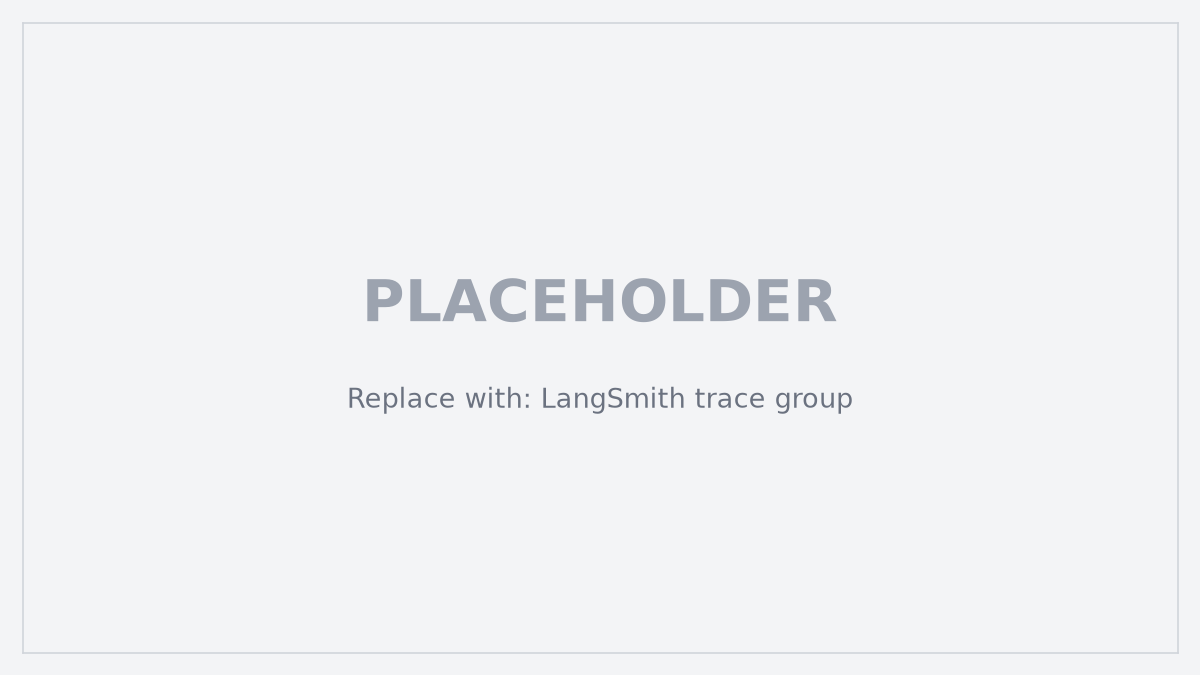
\includegraphics[width=0.7\textwidth]{langsmith-trace.png}
  \caption[LangSmith trace group]{LangSmith trace group for one full
  matching run.}
  \label{fig:langsmith-trace}
\end{figure}

\section{Sprint Retrospective}
\label{sec:s4-retro}

\textbf{What worked:} treating evaluation as its own committed backlog
item (ADQ-27/29/30/33, 20 of the sprint's 35 points) rather than an
informal afterthought is what actually produced defensible numbers:
every metric in ADQ-33 (Implementation, Section~\ref{sec:s4-impl}) has
a real dataset and sample size next to it because measuring it was
planned work, not something squeezed in at the end.

\textbf{What didn't:} the TDR extraction field-level F1 regression test
(as opposed to the simpler document-level pass-rate already reported)
hit a hard timeout under free-tier LLM latency across all 13 real TDR
fixtures run together in one test. The document-level pass-rate
(92.3\%) stood in as the sprint-close proxy; the underlying test was
restructured after sprint close (persisting each fixture's result
independently, so a full run no longer needs to complete all 13 fixtures
uninterrupted) but was not re-run to completion before this report was
written, for the same free-tier-quota reason noted throughout this
report. This is stated here plainly rather than silently left as a gap.
Every free-tier constraint described in this report is a deliberate
zero-budget choice for the internship, not a ceiling on the
architecture itself: \texttt{ModelRouter} already treats the cloud
provider pool as configuration, not code, so a production deployment
backed by a single paid key (a Claude or GPT-class API key) removes the
rotation/quota/latency behavior described here entirely.

\textbf{Change beyond Sprint 4:} the sections below cover real work
completed after this sprint's formal close, in the final days before the
live demonstration. This is not a fifth sprint, since none of it was
planned or story-pointed in advance, but real engineering worth
reporting honestly rather than silently folding into Sprint 4's own
numbers.

\section{Beyond the Sprint --- Post-Close Hardening}
\sectionmark{Post-Sprint Hardening}
\label{sec:post-sprint-hardening}

In the days immediately following Sprint 4's formal close, additional
engineering work was carried out ahead of the internship's live
demonstration. This work was not part of the 170-point backlog above and
was not story-pointed or sprint-planned in advance. It is reported here
separately, and explicitly, so the sprint-by-sprint narrative above
remains an accurate record of what was actually committed and delivered
against a plan, rather than retroactively inflated with unplanned scope.

\begin{description}
  \item[Skill-taxonomy candidate harvesting] A new capability closing a
    real gap in Sprint 2's skill-normalization design (Design,
    Section~\ref{sec:s2-design}): every skill term that fails to match
    the taxonomy is now logged to a new \texttt{skill\_taxonomy\_candidates}
    table with an occurrence count, and a small admin API lets a human
    review and approve or reject pending candidates. Approved terms
    become real taxonomy entries with their own embedding, never
    auto-added. A subtle transactional bug found during code review
    (harvesting ran on the same database transaction as the rest of a
    matching run, so a harvesting failure could have silently rolled
    back an unrelated candidate's already-computed match result) was
    fixed using a SQL savepoint (\texttt{session.begin\_nested()}),
    isolating that one failure mode from the rest of the run.
  \item[Embedding provider fallback] Sprint 1's multi-provider failover
    (Chapter~\ref{chap:sprint-1}) had only ever covered chat/completion
    calls: embeddings had no fallback at all, so a local Ollama outage
    would fail every embedding-dependent code path. The fix
    deliberately does \emph{not} add a blanket fallback everywhere:
    embeddings that get persisted and later compared against other
    persisted embeddings (a CV's stored vector, a taxonomy entry) keep
    no fallback and fail loudly instead, since silently mixing vectors
    from two different embedding models would produce a meaningless
    similarity score that looks valid; embeddings compared only within
    one single operation (TDR chunk retrieval) get a real, sticky
    fallback, since nothing from a different provider is ever compared
    against them.
\end{description}

This work is deliberately excluded from Sprint 4's own story count and
velocity figures above: it is real, but it was not planned, and
presenting it as if it had been would misrepresent this report's own
sprint-by-sprint accounting.

\section{Conclusion}

Sprint 4 closes the four-sprint, 33-story, 170-point product backlog as
fully scoped and delivered.
Where Sprints 1--3 built AdéquIA's matching, scoring, anomaly-detection,
and reporting pipeline, Sprint 4 turned it into a coherent, demoable, and
critically \emph{measured} product: every earlier page rebuilt on a
real design system, seven real evaluation numbers computed and presented
rather than claimed, end-to-end tracing, a first PII-masking pass, and
a release-readiness validation package built from those same real
outputs. Two further defects were found and fixed through the same
live-testing discipline established in Sprint 3 (the duplicate-row bug,
the null-vs-0\% sub-score rendering bug), and one real scope gap,
field-level TDR extraction F1, was left honestly stated rather than
quietly dropped. The post-close hardening above closes out the
internship's engineering effort beyond the formal backlog: a real gap in
Sprint 2's skill-taxonomy design closed, and a second real single point
of failure in Sprint 1's provider failover removed, both reported with
the same discipline as everything before them, real work stated as real
work rather than folded into a sprint's numbers it was never actually
part of.
